\section{\acl{EPS}}
\label{pruneEPS}
In the next section the design option tree for the \ac{EPS} will be pruned. The design option trees for the power source, storage, distribution and regulation and control will be dealt with individually in sections \ref{pruneEPS:Source}, \ref{pruneEPS:Storage} and \ref{pruneEPS:Distribution} respectively.

\subsection{Power Source}
\label{pruneEPS:Source}
Fuel cells have a high specific energy density but were not taken into account as a feasible power source because the amount of reactant they would have to bring for long term mission is too large for microsatellites. Primary batteries were equally unfeasible because of their limited lifetime, which is in the order of minutes to months. Radio isotopes and nuclear fission reactors were discarded because of their high cost and low specific power, as were thermionic and thermoelectric conversion for static power sources.
This leaves photovoltaics and concentrated solar radiation together with an engine in a thermodynamic power cycle.

The pruned design option tree for the powersource can be seen in figure \ref{fig:DOTeps_sourcePruned}

\begin{figure}
\centering
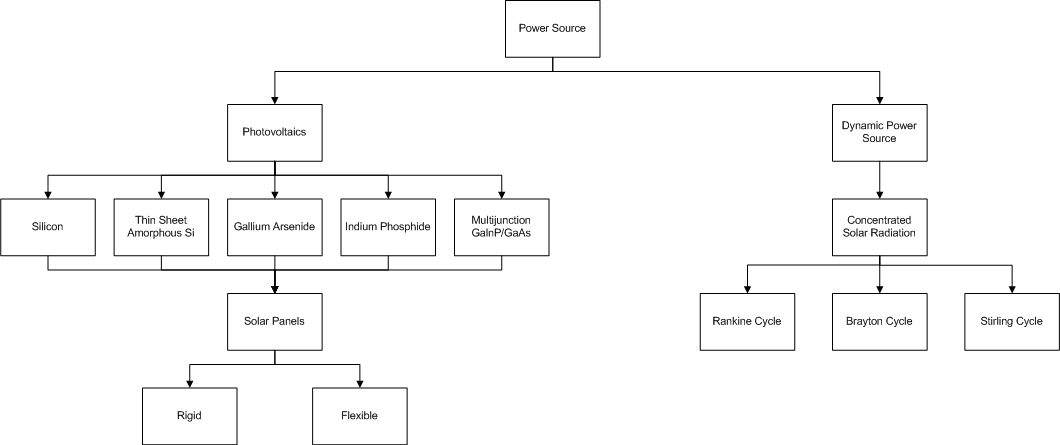
\includegraphics[width=\textheight, angle=90]{chapters/img/DOTeps_sourcePruned.png}
\caption{The pruned design option tree for the power source}
\label{fig:DOTeps_sourcePruned}
\end{figure}

\subsection{Power Storage}
\label{pruneEPS:Storage}
The only obvious candidate for power storage was secondary batteries because, as mentioned before, the lifetime of primary batteries is too short.
Of the most common secondary batteries, sodium-sulfur batteries are not an option for us because their operating temperature of 350 degrees Celsius is too high.

The pruned design option tree for the powersource can be seen in figure \ref{fig:DOTeps_storagePruned}

\begin{figure}
\centering
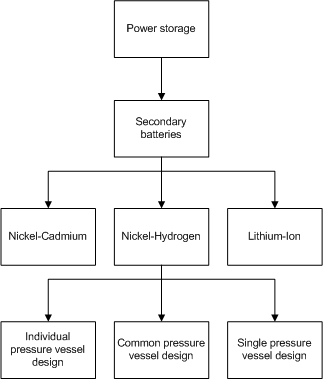
\includegraphics[width=0.35\textwidth]{chapters/img/DOTeps_storagePruned.png}
\caption{The pruned design option tree for the power storage}
\label{fig:DOTeps_storagePruned}
\end{figure}

\subsection{Power Distribution, Regulation and Control}
\label{pruneEPS:Distribution}
For the power distribution, regulation and control there were no obvious non-candidates. Because the power distribution, regulation and control depend on the type of power source, which depends on the payload power requirements, pruning will be done later on after these subsystems have been chosen --- this is done in the tradeoff.

The design option tree for the powersource can be seen in figure \ref{fig:DOTeps_reganddisPruned}

\begin{figure}
\centering
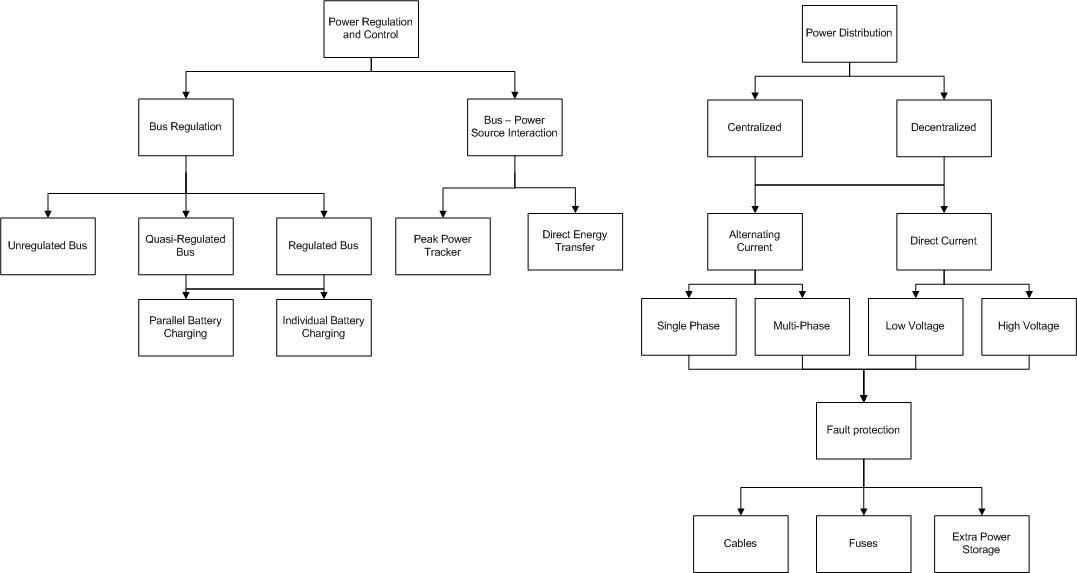
\includegraphics[width=\textheight, angle=90]{chapters/img/DOTeps_reganddisPruned.png}
\caption{The design option tree for the power distribution and regulation and control}
\label{fig:DOTeps_reganddisPruned}
\end{figure}